\chapter{Introduction}%
\label{chapter:introduction}

\begin{introduction}

\end{introduction}

\section{Concept}\label{sec:concept}

\subsection{Basketball Context}\label{subsec:basketball-context}
Portugal is cleary not known for its basketball, the quality is far behind other european countries.
In the International Basketball Federation (FIBA) world ranking\cite{fiba}, Portugal is in the 47 place, and in the middle of the European table in 25th place.
Comparing with our neighbours Spain that is in 7th in the world ranking.
However, in the past years, the portuguese basketball achieve some marks.

First, Portugal had its first player in one of the best women league in the world, ``Ticha'' Penicheiro played during 15 seasons in the WNBA in th USA, winning a title with the Sacramento Monarchs, and some individual awards.
And in 2019, entered the Women’s Basketball Hall of Fame, that has the goal of honouring the most influential players in women basketball.\cite{ticha}

After her, Neemias Queta was drafted to the NBA in 2021, being the first portuguese in the NBA, and in the 2023--24 season won his first title with the Boston Celtics.
Besides not being the most valuable player in his team in the USA, he played an important role with the National team in second appearance in the EuroBasket tournament in 2025.
In this campaign, the portuguese team made a surprise performance, passing through the group phase and then, confronting the German team.
In this game the portuguese team was holding up until the last quarter, where the world champions and the winners of the EuroBasket 2025 took the victory.
After the first victory in the EuroBasket, Neemias mentioned that it was a great moment fot the sport in Portugal and wants the sport to grow more in Portugal.\cite{neemias}
To help with this goal, a survey was made in order to understand how players and basketball enthusiasts use the public basketball courts, the frequency, and the problems.

\subsection{Problem}\label{subsec:problem}

After a some conversations with few basketball players and leaning heavily in a survey responses, basketball players and enthusiasts wish to go more often to public courts.
Besides time constraints, this two scenarios and the following complains are in these players mind:

\paragraph{Key Scenarios}
\begin{itemize}
    \item \textbf{Insufficient players}: people arrive to play but cannot form a team because not enough players are present;
    \item \textbf{Overcrowding}: courts are full, forcing players to wait or leave.
\end{itemize}

\paragraph{Common annoyances reported}
\begin{itemize}
    \item Poor or unpredictable court conditions;
    \item Courts that are either empty or overcrowded;
    \item Social problems between players, including aggressive or unpleasant behaviour, individualistic style, and mismatched competitiveness (players who do not take the game seriously or whose skill and attitude creates a poor experience).
\end{itemize}

These issues point to a coordination and information problem.
Basketball players lack a platform to discover, schedule and evaluate informal games, and to verify court availability and condition.
As a result, players often waste time visiting courts with unsatisfiable condition, which decreases participation and lower quality of both social and sporting experience.

\subsection{Proposed Solution}\label{subsec:proposed-solution}

The proposed solution is to design and implement a digital platform that addresses the coordination and information gaps in amateur basketball in public courts, by focusing on two primary features:

\begin{description}
    \item [Informal Games] ``Pickup games''\footnote{``Pickup games'' is the name used by basketball players to call a game without a formal organization (not in a league, no referee, no strick rules)} -
    Enable players to create, discover and join informal matches (pickup games), with features that support different play modes and social organization:
    \begin{itemize}
        \item Players can create, search for and join games listed on the platform;
        \item The games can be competitive or casual;
        \item Competitive games contribute to a leaderboard/raking table per court;
        \item Game formats include 1v1, 3v3, 4v4, 5v5;
        \item Users can create and mange persistent teams and challenge other teams;
        \item Users can set a team as ``next''\footnote{``next'' is used in the casual pickup games to tell the current teams playing, that wants to play against the winning team.} to a game, to play against the winner.
    \end{itemize}

    \item[Court Availability and condition awareness]
    Provide users with real-time and information about courts so they can decide where and when to play:
    \begin{itemize}
        \item Persistent court catalogue with attributes - name, location, full/half court, number of courts, has water fountain, etc;
        \item Users can indicate intent to attend a court at a specific time, so others can have an idea of the availability;
        \item User can mark themselves ``present'' at a court;
        \item Optional automatic geolocation-based check-in to simplify presence signalling;
        \item Live occupancy indicators to show how many users intend to go and how many are currently present;
        \item Court condition reporting by the users, they can submit short status updates to report issues.
        \item Display short weather summary for the court location (optional)
    \end{itemize}
\end{description}


\section{State of the Technology}\label{sec:state-of-the-technology}

This platform has to reach the maximum basketball players for it to work properly, and should work when the players are in the court, or anywhere.
In order to achieve this, the platform should be access from the mobile phones, and Statcounter\footnote{Statcounter is a company that provides a tool for users to get insights of their website's visitors} Global Stats reports the following about the Mobile Operating System Market Share in Portugal in September 2025: 65.65\% is from Android, and 33.94\% is iOS\cite{statcount}.
Despite the fact that more than half of people uses Android, the goal is still reach the maximum players possible, so the platform should be accessible from Android and iOS phones.

In order to develop a mobile application for both platforms, there are different options of approaches that can be selected for the implementation, which are the native, cross-platform, web, hybrid, modeling, cloud-based and merged approaches\cite{Khachouch2020}.

\subsection{Native Apps}\label{subsec:native-apps}

Going Native, means that the app will be developed with to a specific OS, using its programming language.
To build native Android applications, developers typically use Kotlin or Java.
Both language are compiled to Java Bytecode that runs on the Android Runtime (ART).
As for iOS, developers use Swift or Objective-C, mainly the first one, to build native iOS applications.

With native apps, there is no need for third-party frameworks, as the code is compiled directly into the platform's native language.
This results in better performance and faster execution compare to other solutions, which will be discussed later.
In addition to performance, native development offers security benefits, since developers can take advantage of the built-in security features of the operating system.
When it comes to  User Interface (UI) and User Experience (UX), each platform provides its own guidelines: Android follows Material Design, while iOS follows Human Interface guidelines.
This consistency makes apps easier to navigate, and there is no issues in the app adaptation to other devices.
Finally, native applications can make full use of device features such as the camera, microphone and GPS, which enhances functionality and integration.\cite{Nagy2022}

When the goal is to deliver an application for both Android and iOS using native development, each feature must be implemented twice, once for each platform and in different programming languages.
As Roby Nagy explains in \textit{Simplifying Application Development with Kotlin Multiplatform Mobile}\cite{Nagy2022}, the development cost of this approach can be expressed as:


\[Cost of development (n) = n * FC\]

where \textit{n} represents the number of platforms and \textit{FC} the \textit{feature complexity}, defined as the sum of all sub-features that compose a feature.
The figure \ref{fig:costNative} , taken from Roby Nagy' book \cite{Nagy2022}, illustrates how the development cost grows for two platforms (blue line) and three platforms (red line) as the number of features increases, assuming no cost reduction from sharing code.

\begin{figure}[h]
    \caption{Cost of native development as a function of feature comlpexity \cite{Nagy2022}}
    \centering
    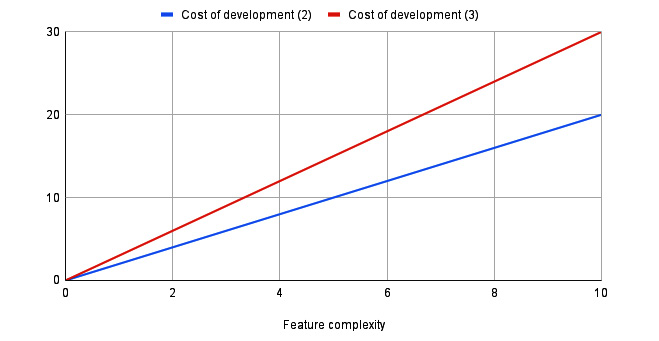
\includegraphics[width=0.5\textwidth]{figs/Figure_1.1_B17614_cost_of_native_dev}
    \label{fig:costNative}
\end{figure}


Beyond this calculation, additional factors complicate native development.
Each platform has distinct characteristics, and a solution that is straightforward to implement on one platform may be unavailable or significantly harder to achieve on another.
This divergence creates extra overhead in aligning features sets across platforms.
So, Nagy introduces the additional component, \textit{Synchronization Cost}, which increases in an exponential way as the number of features and its complexity grows.
The updated formula is expressed as:

\[Cost of development (n) = n * FC + Sync Cost ^ {FC}\]



\subsection{Cross-Platform Apps}\label{subsec:cross-platform-apps}

In order to avoid repeating the same code for different platforms, there are Cross-Platforms approaches.
With this method, it is possible to create applications that run on multiple operating systems.
In a first look, using cross-platform methods can be an effective solution to develop applications for a multiple platforms, when time, cost and basic interoperability is the primary concern.
On the other hand, Cross-Platform applications tend to have the worst performance and user experience compared with Native apps, as they are behind the evolution of Android and iOS and cannot take full advantage of each platform's features\cite{Nagy2022}.
Here are the different approaches to develop Cross-Platform applications.

\subsubsection{Web Applications}

Any application that is access through \textit{HTTP} requests over a network is called a web based application.
These applications are implemented with HTML, CSS and JavaScript.
Until Progressive Web App appeared, these applications were browser only, but now, they can be installed in the device, can have offline availability, push notifications and background sync, also able to run on desktop.
Developers normally use Angular or React, and other frameworks are StencilJS or Svelte.
However, PWAs cannot access key platform's features as the Native apps can, and also, has a possible higher energy consumption.\cite{Huber2021}


















